\begin{rightcolumn}

\subsubsection{Valor en las condiciones actuales.}

Se utilizó una metodología de valuación de negocios basada en el punto número 2 del pentágono de explotación de oportunidades, conocido como \textit{valor actual interno}. Lo anterior  implica realizar el análisis de valor del activo intangible en las condiciones que opera al día de hoy; esto es, sin realizar ninguna explotación de oportunidades en los factores internos y externos. (\autoref{fig:hexagono})\\

``\textcolor{secundario}{Valor en las condiciones actuales.} Es el valor de la unidad econ\'omica valuado en las condiciones que opera al d\'ia de hoy, esto es, sin realizar ninguna explotaci\'on de oportunidades en los factores internos y externos. Este valor resulta de la aplicaci\'on de un trabajo valuatorio para determinar el valor de la unidad econ\'omica en sus condiciones actuales.'' \\



\end{rightcolumn}
\begin{leftcolumn}

\begin{figure}[H]
\centering
\caption{Pent\'agono de Explotaci\'on de oportunidades\label{fig:hexagono}}
\includegraphics[width=5cm]{\rutaImagenes/pentagono}\\
Fuente:Valuation. Copeland Tom, Koller Tim y Murrin Jack.\\

John Wiley \& Sons. 2000.
\end{figure}

\end{leftcolumn}




